% ACS manuscript class, journal identifier jcisd8.
\PassOptionsToPackage{hyphens}{url}
\documentclass[journal=jcisd8,manuscript=article,layout=twocolumn]{achemso}
\usepackage{amsmath,graphicx,booktabs,tabularx,array}
\usepackage{url}
\usepackage{hyperref}
\hypersetup{hidelinks}
\emergencystretch=2em
\setcounter{dbltopnumber}{2}
\renewcommand{\dbltopfraction}{.90}
\renewcommand{\textfraction}{.07}
\renewcommand{\dblfloatpagefraction}{.75}
\setkeys{acs}{articletitle=true,doi=true}
\title{Coordination Constraints and Information Content in Predicting Lewis Acidity}
\author{Simin Huang}
\email{hsm24@mails.tsinghua.edu.cn}
\affiliation{Tanwei College, Tsinghua University, Beijing 100086, China}
\author{Shenqi Zong}
\affiliation{Tanwei College, Tsinghua University, Beijing 100086, China}
\author{Han Chen}
\affiliation{Tanwei College, Tsinghua University, Beijing 100086, China}
\begin{document}
\begin{abstract}
Molecular geometry and electronic descriptors provide complementary routes to predicting the fluoride ion affinity (FIA) of Lewis acids, but their value depends on coordination constraints and the information available about binding. Across 48,986 FIA49k molecules, DimeNet++ achieves a main-test MAE of 11.21 $\pm$ 0.27 kJ\,mol$^{-1}$ over three training seeds, with ensemble analysis showing the largest absolute gain over released connectivity predictions for tridentate ligand environments. P(III) compounds remain difficult across acid-geometry representations, whereas refinement of a PBEh-3c acid--fluoride calculation gives MAE 3.44 kJ\,mol$^{-1}$ for this class and 3.29 kJ\,mol$^{-1}$ overall, retaining 3.35 kJ\,mol$^{-1}$ on held-out ligand-scaffold combinations. Paired molecular structures reveal a second, distinct sensitivity: the loss of accuracy upon changing geometry source is concentrated in acids whose optimized structures disagree, connecting chemical coordination, quantum refinement and structural provenance in the choice of an FIA prediction workflow.
\end{abstract}
\section{Introduction}

Lewis acids participate in bond activation, catalysis and anion recognition, making the prediction of their binding strength a useful objective for molecular design. Fluoride ion affinity (FIA), defined as the negative enthalpy change for binding F$^-$ to a Lewis acid, provides a quantitative measure of affinity toward a hard Lewis base. Accurate quantum-chemical FIA calculations have established trends across the p-block, but their use in large-scale screening is limited by the cost of evaluating both the free acid and its fluoride adduct. \cite{sigmund2024fia,erdmann2020fia} Predictive models can reduce this burden if their molecular inputs and chemical range match the intended screening task.

The FIA49k dataset extends FIA prediction across central elements, oxidation states and ligand environments. FIA-GNN demonstrated that molecular connectivity supports prediction in this broad chemical space. \cite{sigmund2024fia} Complementary work on boron Lewis acids showed that chemically informed descriptors can achieve high accuracy within selected scaffold families and can connect predictions to substituent effects. \cite{fenogli2025boron} These approaches address different regimes of chemical diversity. An outstanding question is how much additional information is provided by an optimized acid geometry or by electronic quantities obtained from the same calculation, particularly when the ligand framework changes.

Geometric neural networks offer several ways to represent an optimized structure. Equivariant feature messages, directional message passing and continuous distance filters incorporate spatial information through different constructions. \cite{satorras2021egnn,gasteiger2020dimenet,schutt2017schnet} Their predictive performance depends on both representation and optimization, while the molecular distances available to each architecture can also encode angular relationships. A complementary route is $\Delta$-learning, in which a model predicts the difference between an inexpensive quantum calculation and a higher-level reference. \cite{ramakrishnan2015delta} For FIA, this route retains the thermochemical information in a lower-level acid--fluoride binding calculation and changes the information available to the learner.

Here we compare these routes on FIA49k using fixed molecular identities and validation-based model selection. Repeated geometric-model training establishes the effect of representation and readout, and descriptor controls quantify the contribution of acid electronic information. A separate ligand-scaffold partition tests transfer across structural combinations. We then analyze reference-method corrections at matched ligand identity and evaluate the response of frozen models to a change in geometry source. Together, these experiments relate prediction accuracy to the information required by each workflow.

\section{Computational methods}

\subsection{Dataset and structural partitions}

The target is the gas-phase fia\_\allowbreak{}gas-DSDBLYP value from FIA49k, expressed in kJ\,mol$^{-1}$. The reference combines RI-DSD-BLYP-D3(BJ)/def2-QZVPP single-point energies with PBEh-3c structures and the published thermochemical and reference conventions. \cite{sigmund2024fia,fia49ktargets} Targets, geometries and released FIA-GNN predictions were obtained from the versioned Figshare archives. \cite{fia49ktargets,fia49kgeometries,fia49kpredictions} Geometric predictors receive one optimized unbound-acid structure per molecule. The dataset contains 48,986 molecules, 22 atomic species and a maximum of 118 atoms; 13 elements occur as accepting centers. Source checksums, geometry parsing and the complete atom vocabulary are documented in the Supporting Information (SI).

The primary partition contains 32,333 training and 7,001 validation molecules. Six published test groups are evaluated separately: the main FIA44k test (6,732 molecules), CSD compounds (1,200), bimacrocycles (763), four-membered-ring compounds (911), phase-transfer catalysts (15) and additional catalysts (31). All molecules in each group are retained. The CSD source also contributes training and validation compounds, whereas the two small catalyst groups provide individual chemical case studies. Molecular identifiers and reference targets are aligned before calculating any model comparison.

A secondary partition groups the original training, validation and main-test pool of 46,066 molecules by ligand structure. The accepting center is removed from the grouping key. Cyclic ligands are represented by generic Bemis--Murcko scaffolds, and acyclic ligands by generic full graphs. The sorted multiset of ligand representations defines a group; a fixed-seed hash assigns whole groups to training, validation and test with nominal probabilities 0.70, 0.15 and 0.15. This produces 33,460/6,379/6,227 molecules across 12,448 groups. The test therefore holds out complete scaffold combinations, while individual components can occur in other combinations. The SI also reports an exact-ligand-set partition. Models used on these secondary partitions are fitted independently.

\subsection{Representations, controls and training}

The geometric models use trainable atomic-number embeddings and 5.0 Å radius graphs. The EGNN feature-message baseline has seven residual layers of width 128 and retains fixed coordinates, as in the upstream QM9 implementation. \cite{satorras2021egnn} The radial-filter model has four width-128 interaction layers, 32 Gaussian radial functions and a cosine cutoff envelope. \cite{schutt2017schnet} Its sum readout is compared with a readout concatenating the accepting-center, mean and sum representations. The accepting center follows the archive's first-atom convention, checked against the recorded central element. DimeNet++ uses four interaction blocks, hidden width 128, interaction width 64, seven spherical and six radial basis functions; its neighbor cap is 118. \cite{gasteiger2020dimenet} Full architecture settings are provided in the SI.

Each geometric model is initialized from scratch and trained with AdamW, normalized L1 loss, learning rate 0.001 and weight decay 10-6. Learning rates are reduced after eight epochs without validation improvement, with a maximum of 100 epochs and early-stopping patience of 25 epochs. Batch sizes are 64, except for DimeNet++ (32). The checkpoint with the lowest validation MAE is selected for each of three random seeds. Training-derived normalizers, molecular identities and model settings are stored with each checkpoint.

The composition control uses the radial architecture on a complete graph with all distances set to zero. An acid-QM extension combines the geometric readout with six PBEh-3c acid properties: Mulliken and Löwdin center charges, dipole magnitude, global electrophilicity, and HOMO and LUMO energies. Four numerical chemical metadata fields are included in the same global input. A composition-plus-QM control receives these global quantities without coordinates. Feature imputation and standardization are fitted on training molecules. These extensions test the additional value of electronic information available from the acid calculation.

Classical controls use histogram-based gradient boosting (HGB). Inputs comprise chemical metadata, 190 varying RDKit 2D descriptors, the six acid electronic quantities, or their combinations. \cite{rdkit,pedregosa2011sklearn} Metadata encode the central element, oxidation state, period, group, ligand count and denticity. HGB uses learning rate 0.05, at most 31 leaves and L2 regularization 1. Predictions at 100, 400 and 1,000 fitted stages are compared on the designated validation set. Descriptor filtering is based on training data, and nonfinite values are handled as missing inputs. Released FIA-GNN predictions provide a published connectivity-based reference with its original training procedure. \cite{fia49kpredictions}

\subsection{Quantum correction and statistical analysis}

For quantum-assisted refinement, the learned target is the difference between DSD-BLYP and PBEh-3c FIA. The final estimate is

\begin{equation}
\widehat{\mathrm{FIA}}_{\mathrm{DSD}}=\mathrm{FIA}_{\mathrm{PBEh\text{-}3c}}+f_{\theta}(\mathbf{x}).
\end{equation}

The HGB correction receives lower-level FIA, metadata, RDKit descriptors and the acid electronic quantities. Controls comprise raw PBEh-3c FIA, a global mean correction, center-class mean corrections and a metadata-based HGB correction. All correction parameters are learned from training data, and the same stage-selection budget is used throughout. The lower-level FIA requires both acid and fluoride-adduct calculations, whereas the geometric and acid-QM models require the unbound acid alone. This distinction defines two computational input regimes.

MAE, RMSE, signed error and pooled $R^2$ are evaluated on identical molecular target vectors. Neural results are reported as the mean and sample standard deviation across training seeds; an unweighted prediction ensemble is evaluated separately. Paired bootstrap intervals use 2,000 resamples stratified by central-atom class. These intervals condition on the fitted weights and preserve the composition of each test group. Matched-ligand method comparisons use training molecules only: repeated records are averaged within each ligand-set/center-class cell before pairing central elements.

Geometry-source sensitivity is measured by substituting GFN2-xTB acid structures for PBEh-3c structures while retaining the frozen radial-center models, target values and molecular identities. Radius graphs are recalculated for the alternate coordinates. This evaluates a change in the input-generation protocol; each molecule still contributes one optimized structure. Explicit conformer-ensemble learning involves a different data representation and aggregation problem. \cite{zhu2024marcel} Paired acid/adduct diagnostics in the SI additionally quantify changes in heavy-atom pair distances after checking atom-count and element-order correspondence.

\section{Results and discussion}

\subsection{Geometric information improves broad-space prediction}

DimeNet++ gives the lowest mean MAE among the geometric models, 11.21 $\pm$ 0.27 kJ\,mol$^{-1}$ on the 6,732-molecule main test (Table 1). The EGNN feature-message baseline gives 12.08 $\pm$ 0.16, while the radial models give 12.22 and 12.39 with center and sum readouts, respectively. The three-seed DimeNet++ ensemble reduces MAE to 10.29, compared with 12.11 from released FIA-GNN predictions. The paired bootstrap interval for this ensemble difference is -2.06 to -1.59 kJ\,mol$^{-1}$. The published connectivity reference and the new geometric models have different optimization histories, so this comparison describes the resulting prediction workflows.

\begin{table*}[t]
\centering\small
\caption{Main-test MAE in kJ\,mol$^{-1}$. Geometric-model values are three-seed mean $\pm$ sample SD; composition controls use one seed. Ensemble errors are calculated from averaged predictions. FIA-GNN uses released predictions.}
\begin{tabularx}{\textwidth}{@{}>{\raggedright\arraybackslash}p{.30\textwidth}>{\raggedright\arraybackslash}Xrr@{}}
\toprule
Model & Inputs & MAE & Ensemble MAE \\ \midrule
FIA-GNN & Connectivity & 12.11 & --- \\
HGB metadata & Metadata & 37.57 & --- \\
HGB RDKit & Metadata + 2D & 18.73 & --- \\
HGB acid QM & Metadata + acid QM & 23.02 & --- \\
HGB 2D + acid QM & Metadata + 2D + acid QM & 17.35 & --- \\
Composition control & Composition & 28.70 & 28.70 \\
EGNN feature messages & Acid geometry & 12.08 $\pm$ 0.16 & 11.04 \\
DimeNet++ & Acid geometry & 11.21 $\pm$ 0.27 & 10.29 \\
Radial, sum readout & Acid geometry & 12.39 $\pm$ 0.11 & 11.22 \\
Radial, center readout & Acid geometry & 12.22 $\pm$ 0.17 & 11.15 \\
Composition + acid QM & Composition + QM & 20.16 & 20.16 \\
Geometry + acid QM & Acid geometry + QM & 12.18 $\pm$ 0.04 & 11.12 \\
\bottomrule
\end{tabularx}
\end{table*}

The composition control has MAE 28.70 kJ\,mol$^{-1}$, showing the value of spatial information within the radial-model comparison (Figure 1a). Acid electronic quantities partly recover this information: composition plus acid QM gives 20.16. Combining acid QM with geometry gives 12.18 $\pm$ 0.04, close to the geometric radial model alone. Thus geometry and acid electronic descriptors supply overlapping predictive information in this architecture. The composition control does not contain bond connectivity; the released FIA-GNN results demonstrate the additional information available from a connectivity representation.

\begin{figure*}[t]
\centering
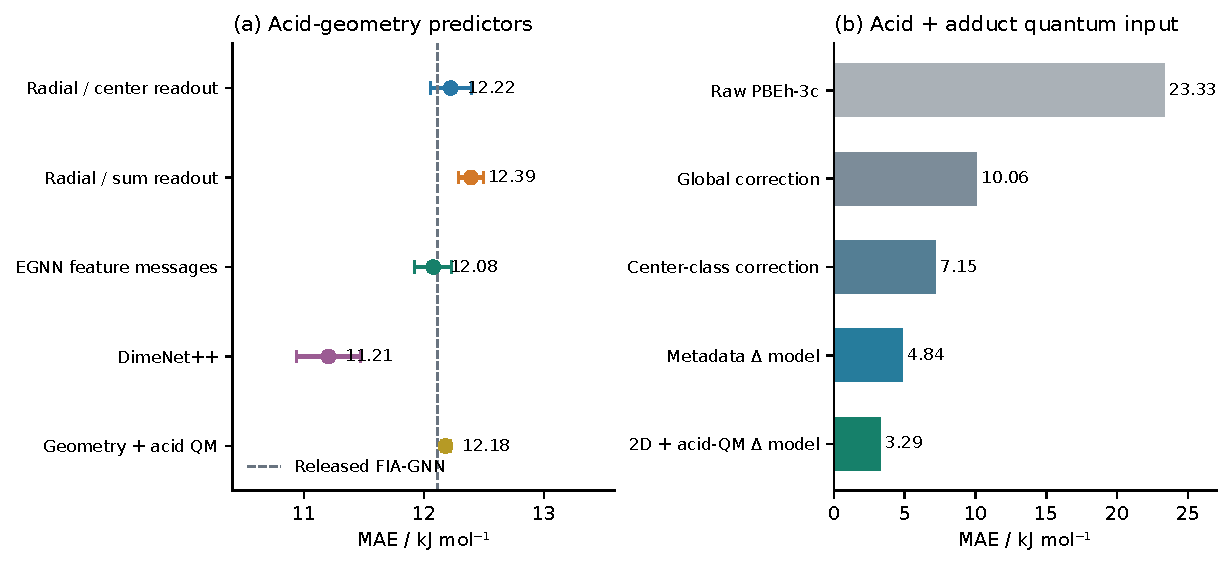
\includegraphics[width=.96\textwidth]{figures/representation_and_refinement.pdf}
\caption{Main-test prediction errors. (a) Acid-geometry models, with mean MAE $\pm$ sample SD across three seeds; the dashed line marks released FIA-GNN predictions. (b) Adduct-dependent quantum correction, compared with raw PBEh-3c FIA and training-derived bias controls. The panels correspond to different computational inputs.}
\label{fig:representation_and_refinement}
\end{figure*}

Errors vary substantially across the published chemical groups (Figure 2). Bimacrocycles remain challenging: released FIA-GNN predictions have MAE 24.08 kJ\,mol$^{-1}$, compared with 20.76 for the DimeNet++ ensemble and 19.89 for the acid-QM ensemble. The main-test advantage of DimeNet++ therefore does not yield a uniform ordering across all structural groups. Central-class results in the SI provide sample counts and target variances alongside errors. The catalyst sets, with 15 and 31 compounds, are useful checks of individual examples but give limited precision for population-level comparisons.

\begin{figure*}[t]
\centering
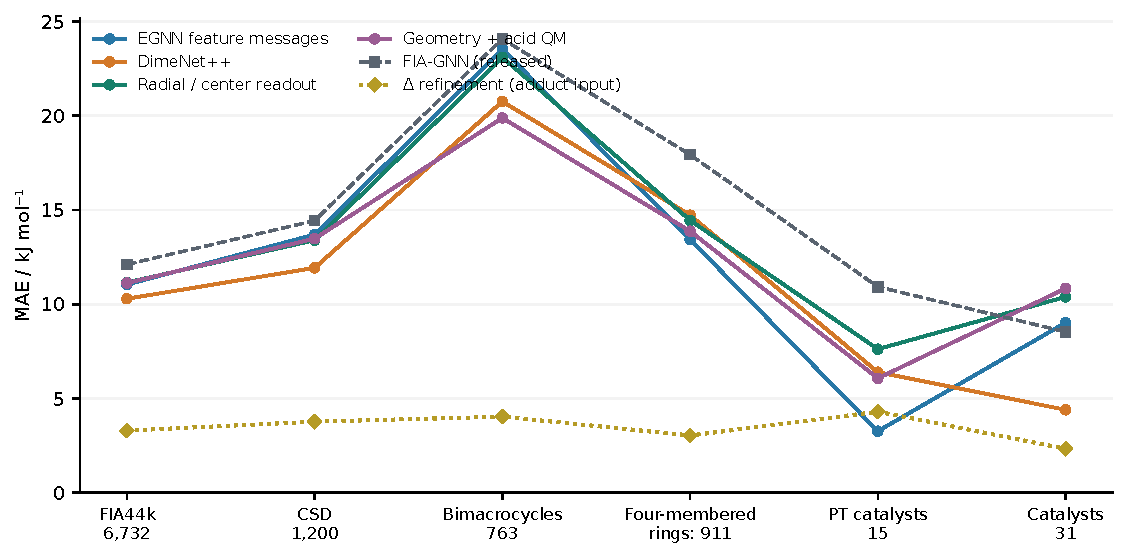
\includegraphics[width=.96\textwidth]{figures/external_groups.pdf}
\caption{MAE across the six published test groups. Geometric and acid-QM predictions are unweighted three-seed ensembles; FIA-GNN uses released predictions. The acid-plus-adduct correction is shown as a separate input regime. Group sample sizes are indicated below the axis.}
\label{fig:external_groups}
\end{figure*}

\subsection{Reference-method correction captures a systematic chemical component}

Raw PBEh-3c FIA has main-test MAE 23.33 kJ\,mol$^{-1}$ and signed error -23.04. A global training-set correction lowers MAE to 10.06; center-class corrections lower it further to 7.15 (Figure 1b). A substantial part of the reference-method discrepancy is therefore shared across molecules and varies with the accepting-center class. The metadata model reaches 4.84, and the full descriptor correction reaches 3.29, with RMSE 4.49 and $R^2$ 0.9965. Molecular descriptors improve on the class mean by resolving variation within each coordination environment.

\begin{table*}[t]
\centering\small
\caption{Quantum-correction MAE in kJ\,mol$^{-1}$ across the official test groups. All corrections are fitted on training molecules; every row uses lower-level acid-plus-adduct FIA.}
\begin{tabularx}{\textwidth}{@{}>{\raggedright\arraybackslash}p{.30\textwidth}rrrrrr@{}}
\toprule
Model & Main & CSD & Bimacro & Ring-4 & PT & Catalysts \\ \midrule
Raw PBEh-3c & 23.33 & 26.73 & 29.76 & 26.64 & 14.19 & 14.63 \\
Global correction & 10.06 & 10.67 & 11.31 & 10.00 & 9.78 & 9.74 \\
Center-class correction & 7.15 & 8.41 & 8.33 & 6.82 & 3.23 & 6.82 \\
Metadata $\Delta$ model & 4.84 & 6.94 & 5.00 & 3.79 & 5.37 & 3.21 \\
Full descriptor $\Delta$ model & 3.29 & 3.77 & 4.03 & 3.03 & 4.30 & 2.32 \\
\bottomrule
\end{tabularx}
\end{table*}

The central-element trend persists when ligand identity is controlled (Figure 3). For 34 training ligand sets shared by P(III) and As(III), the DSD-BLYP--PBEh-3c correction is on average 2.66 kJ\,mol$^{-1}$ larger for As(III), with a paired bootstrap interval of 0.84--4.62. The corresponding differences are 6.40 kJ\,mol$^{-1}$ for 98 Ge(II)/Sn(II) pairs and 6.35 kJ\,mol$^{-1}$ for 103 Sn(II)/Pb(II) pairs. Some neighboring-center contrasts have intervals spanning zero. These matched comparisons show that the class dependence is not explained solely by different ligand populations, while remaining descriptive comparisons between computational reference levels.

\begin{figure*}[t]
\centering
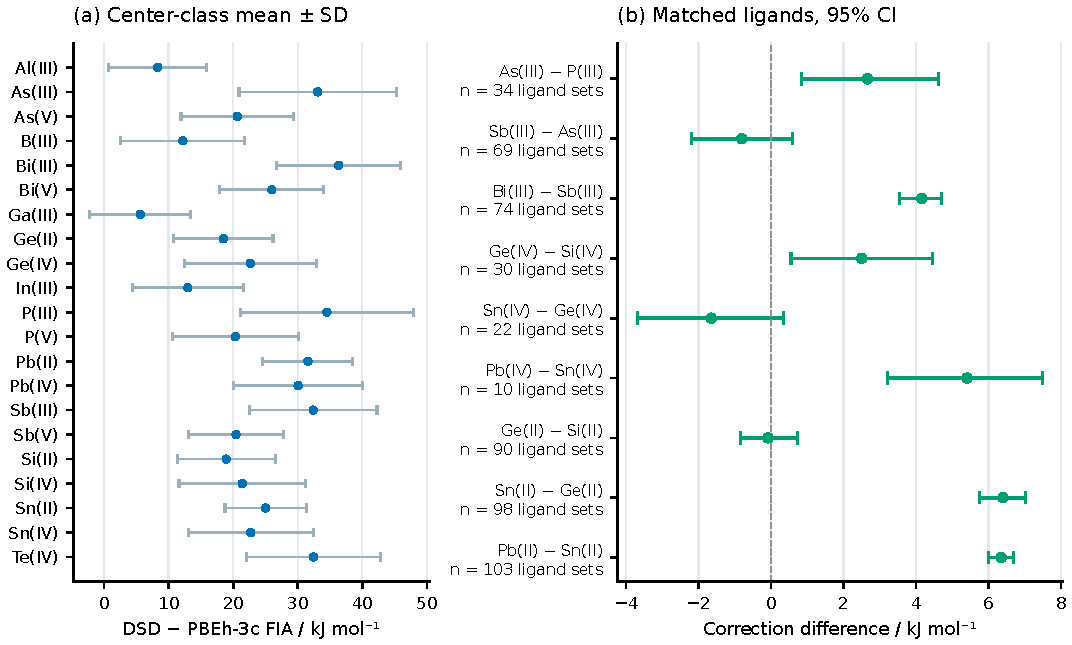
\includegraphics[width=.80\textwidth]{figures/method_corrections.pdf}
\caption{Chemical dependence of the reference-method correction in training data. (a) Center-class means of FIA(DSD-BLYP) - FIA(PBEh-3c), with within-class SD. (b) Paired correction differences between neighboring central elements at identical canonical ligand sets, with 95\% ligand-set bootstrap intervals. All nine declared contrasts and their sample sizes are shown.}
\label{fig:method_corrections}
\end{figure*}

The full correction remains accurate across the external groups, with MAE 3.77 kJ\,mol$^{-1}$ for CSD molecules, 4.03 for bimacrocycles and 3.03 for four-membered rings (Table 2). In these groups, the low-level binding calculation supplies acid/adduct information that is absent from an acid-only representation. The practical benefit is consequently greatest when a PBEh-3c FIA calculation is already available and a more expensive reference-level estimate is required.

\subsection{Transfer across ligand scaffolds and geometry sources}

On the secondary ligand-scaffold multiset partition, the radial-center model gives MAE 12.77 $\pm$ 0.13 kJ\,mol$^{-1}$, compared with 19.10 for the independently fitted RDKit control. Acid-QM fusion gives 12.75 $\pm$ 0.03. The quantum correction gives 3.35, versus 7.25 for the center-class correction. These results support transfer across complete ligand-scaffold combinations in the defined partition. Individual scaffold components and central elements remain shared, so this test probes a different generalization problem from prediction for entirely new ligands or elements. DimeNet++ is evaluated on the official partition only.

Changing the geometry-generation method produces a distinct source of error. With the radial-center ensemble frozen, substitution of GFN2-xTB acid structures increases main-test MAE from 11.15 to 13.02 kJ\,mol$^{-1}$ (Figure 4). The target values and molecular identities are unchanged. The difference therefore measures the consequence of supplying a deployed model with a different structural input distribution. It also shows why geometry provenance belongs in the model specification: a cheaper geometry protocol cannot be assumed to preserve the accuracy measured on the training geometry domain.

\begin{figure*}[t]
\centering
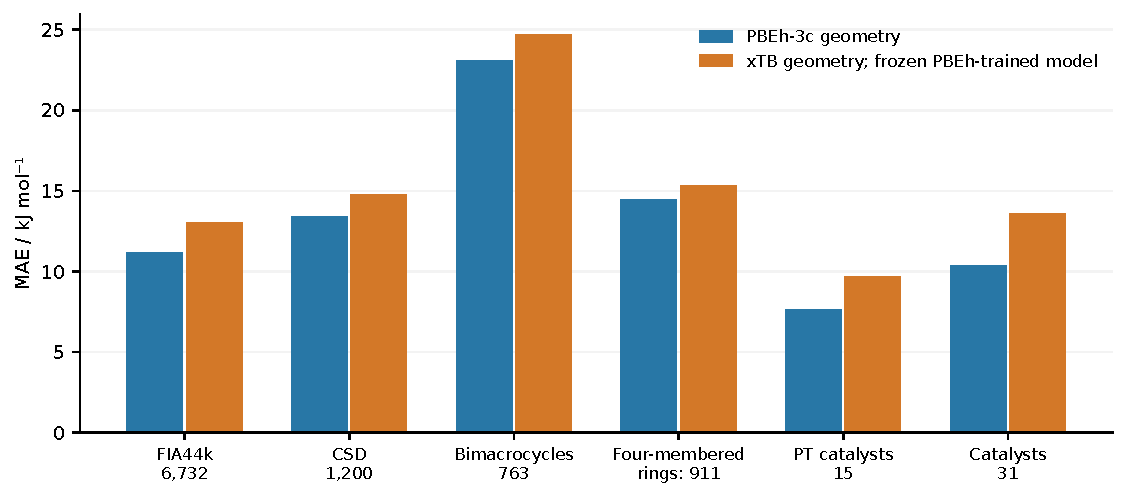
\includegraphics[width=.96\textwidth]{figures/geometry_source_shift.pdf}
\caption{Geometry-source sensitivity of the frozen radial-center ensemble. Blue bars use PBEh-3c acid geometries; orange bars use corresponding GFN2-xTB geometries with the same model weights and targets. Radius graphs are recalculated for each structure.}
\label{fig:geometry_source_shift}
\end{figure*}

\subsection{Chemical interpretation and practical scope}

FIA reflects the relative enthalpies of the free acid and the fluoride adduct. Acid geometry can encode preorganization and local coordination, while a lower-level FIA additionally includes the energetic response to binding. This distinction helps explain the different prediction regimes: acid-only models estimate binding from reactant information, whereas the correction model refines an existing binding calculation. Acid/adduct pair-distance changes in the SI quantify structural reorganization, but an energetic decomposition would require consistent calculations of acid deformation, acid--fluoride interaction and thermochemical corrections.

All errors reported here measure agreement with the FIA49k computational reference. Independent FIA benchmarks show that basis-set diffuseness and anchor-point conventions can affect the reference values. \cite{lehmann2025fia} Moreover, Lewis-acid rankings can change with the probe base. \cite{mahdian2026base} The present models are therefore appropriate to the stated gas-phase fluoride-binding endpoint; extension to other bases or experimental catalytic behavior requires corresponding validation. Explicit conformer sampling and independent reference calculations would address additional sources of uncertainty beyond the structural and geometry-source tests considered here.

\section{Conclusions}

The information supplied to an FIA predictor determines both its accuracy and its role in a screening workflow. Geometric models give useful predictions from an optimized acid structure, with DimeNet++ performing best among the representations tested on the official partition. Acid electronic descriptors add little to the tested radial model on average, whereas lower-level acid--adduct binding information enables substantially more accurate reference-level correction. The persistence of this gain across held-out ligand-scaffold combinations, together with the matched-ligand central-element trends, supports quantum refinement as a practical route when low-level FIA is available. Geometry-source sensitivity provides a complementary deployment criterion for acid-only predictors. These results connect model selection to the molecular information available in each screening workflow.

\begin{suppinfo}
Dataset and geometry provenance, partition definitions, neural configurations, seed and ensemble errors, classical controls, paired uncertainty, geometry-source tests and matched-ligand reference-method corrections (PDF).
\end{suppinfo}

\section*{Data availability}
FIA49k targets, geometries and released FIA-GNN predictions are available under CC BY 4.0 from Figshare. \cite{fia49ktargets,fia49kgeometries,fia49kpredictions} Code, frozen models, complete predictions, split manifests and training configurations are available at \url{https://github.com/PeanutUp/Lewis-Acidity-Prediction}. Source archives and restored artifacts are verified by checksums.
\section*{Acknowledgements}
OpenAI Codex was used for manuscript editing, code development, computational experiment execution and analysis-script preparation.

\bibliography{references}
\begin{tocentry}
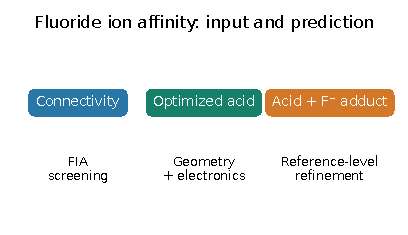
\includegraphics[width=3.00in]{figures/toc_graphic.pdf}
\end{tocentry}
\end{document}
